
\chapter{Proposed approach}

\label{Chapter4}

%----------------------------------------------------------------------------------------

In the previous chapters we have introduced the key components of the approach we followed in our study: on the one hand, we have described existing satellite image datasets and introduced the actual data we will consider, and on the other, we have discussed Deep Learning, how it works and how we can use it for our problem. Now, we are ready to describe our approach: the image feature extraction, the model architecture and the training scenario.

\section{Image features and transfer learning}\label{sec:transferLearning}

In order to train a model based on images, some sort of features need to be extracted. Traditionally, this image feature extraction was based on a set of hand-crafted detectors aimed to detect edges, corners, blobs and other feature descriptors. Some of these detectors are the Sobel filter, Laplacian of Gaussian (LoG), Difference of Gaussians (DoG), Determinant of Hessian (DoH), SIFT \parencite{Lowe1999,Lowe2004}, SURF \parencite{Bay2006}, Histograms of Oriented Gradients (HOG) \parencite{Dalal2005} and Gabor filters.

\begin{figure}[h!]
	\centering
	\begin{subfigure}{.5\textwidth}
  		\centering
  		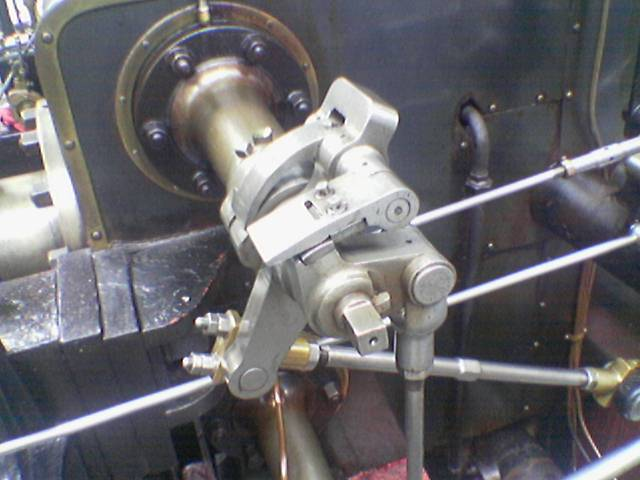
\includegraphics[width=.9\linewidth]{sobel_valve_original.png}
	\end{subfigure}%
	\begin{subfigure}{.5\textwidth}
  		\centering
  		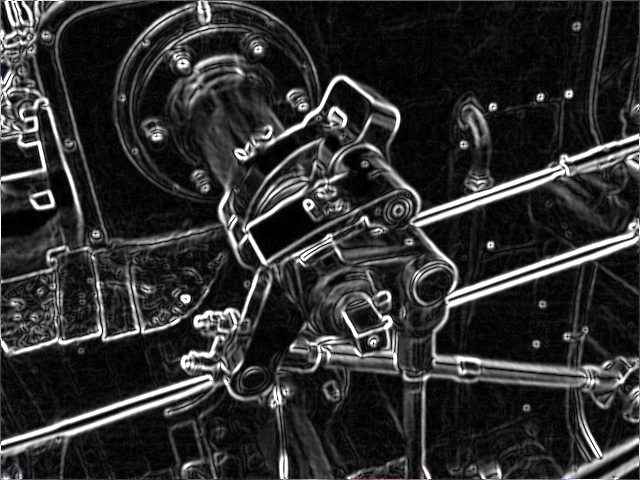
\includegraphics[width=.9\linewidth]{sobel_valve_processed.png}
	\end{subfigure}
	\captionsetup{width=1\linewidth}
	\caption{\textbf{Example of the Sobel filter.} The Sobel operator uses an approximation of the gradient of the image intensity at each point to detect and emphasize edges.}
	\label{fig:sobel}
\end{figure}

\begin{figure}[h!]
	\centering
	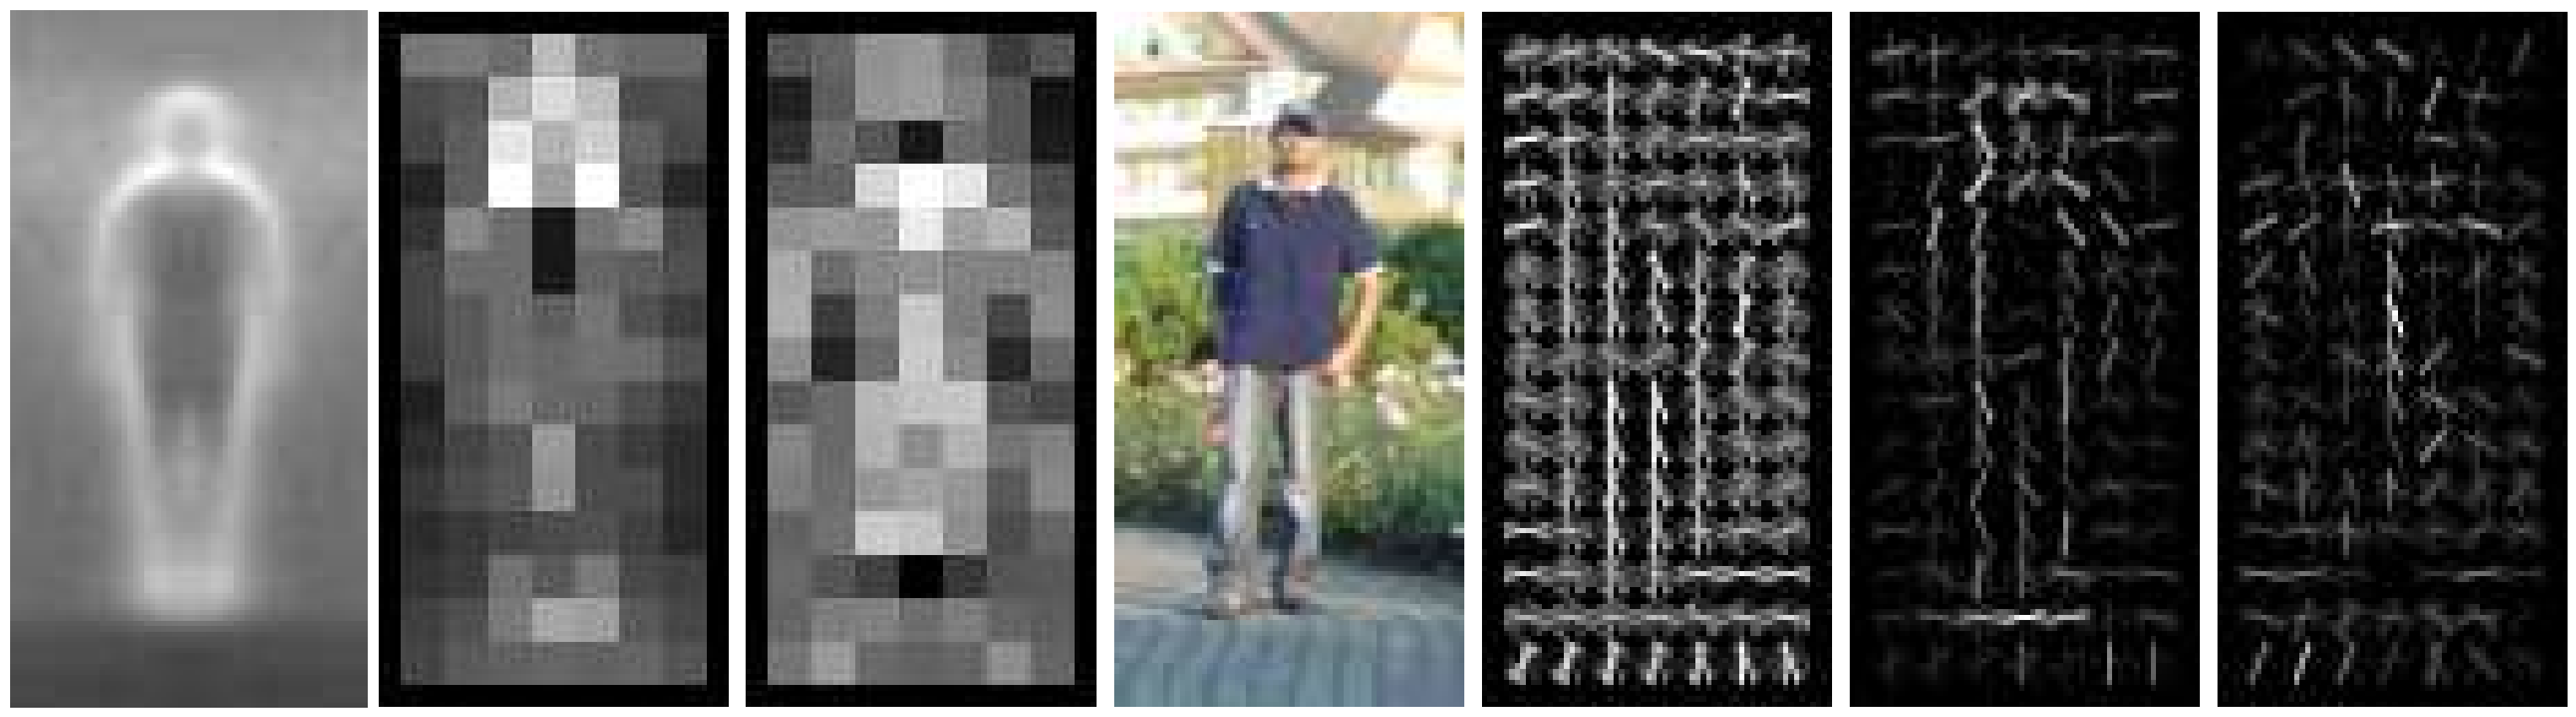
\includegraphics[width=0.9\textwidth]{Figures/hog_example.png}
	\captionsetup{width=1\linewidth}
	\caption{\textbf{Examples of HOG detector \parencite{Dalal2005}.} A histogram of intensity gradient orientations is computed in a dense grid of cells, which gives a measure of the shapes in the image.}
	\label{fig:hog}
\end{figure}

More recent approaches to image classification using Neural Networks have benefited from the existing and increasing computational power, and deep Convolutional Neural Networks have been able to achieve higher performance than traditional models. 

Yet, training a deep CNN from scratch for a particular problem requires a large and exhaustive dataset along with a huge amount of computational power. However, it has been shown that the architectures of pre-trained NN can be reused for other purposes and achieve equally great performance. This is known as \textbf{Transfer Learning}. Figure \ref{fig:transfer_learning_idea} schematizes this idea. These pre-trained architectures can be re-purposed by reusing the learned weights and either replacing the final layers of the net by some other classifier, or even fine-tuning all the layers for the specific problem. In any case, the initial layers of the Neural Network provide a great image feature extractor.

\begin{figure}[h!]
	\centering
	\captionsetup{width=1\linewidth}
	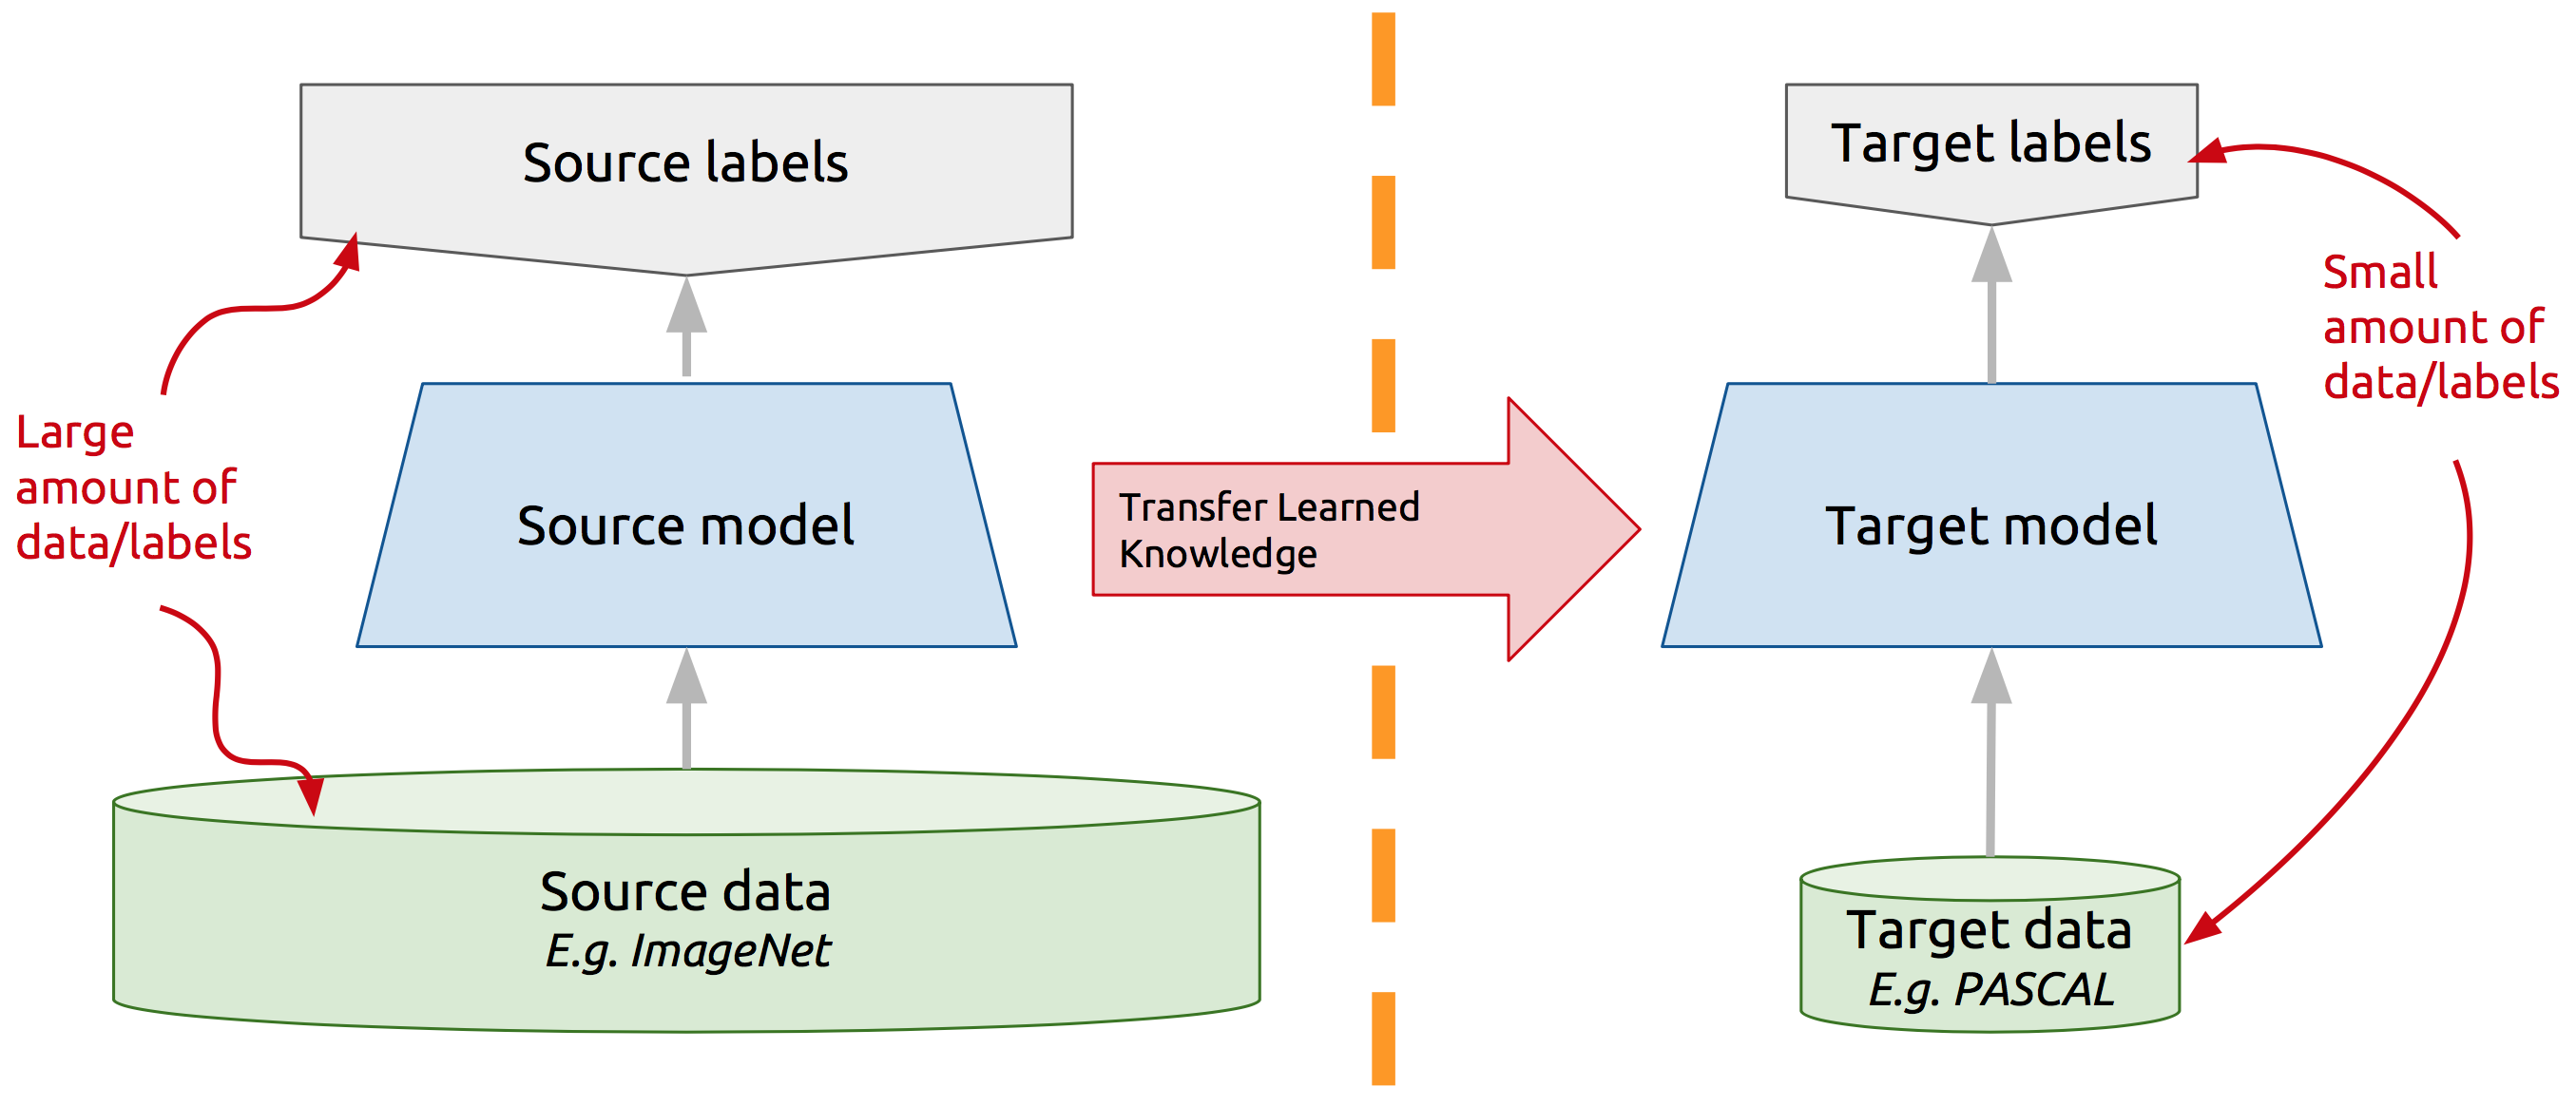
\includegraphics[width=1\textwidth]{Figures/transfer_learning_idea.png}
	\caption{\textbf{Transfer Learning}: a model learned from a large dataset can be transferred and reused for another purpose. \parencite{McGuinness2017}}
	\label{fig:transfer_learning_idea}
\end{figure}

In the next section we describe our approach using transfer learning from a ResNet architecture.

%Consequently, there is an increasing library of available pre-trained models and weights: Xception, VGG, InceptionV3, ResNet.
%Most of these models have weights pre-trained on ImageNet, a large dataset containing more than 14 million hand-annotated images and over 20.000 categories.

%\begin{figure}[h!]
%	\centering
%	\captionsetup{width=1\linewidth}
%	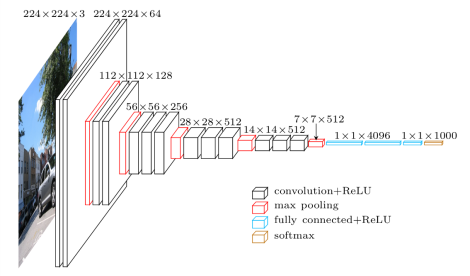
\includegraphics[width=1\textwidth]{Figures/imagenet_vgg16.png}
%	\caption{\textbf{VGG16 architecture}. Stack of $3\times 3$ convolutional and max pooling layers.}
%	\label{fig:degrade}
%\end{figure}

%\subsection{ResNets}

%Experience with Neural Networks, and CNN in particular, show that deeper nets tend to perform better, as these are more capable to model higher complexity. Yet, at some depth point, training becomes too difficult, because the gradient values obtained from the loss function are lost after several layers. This is known as \textbf{vanishing gradient}. ResNet fixes this is issue with Residual...

\section{Proposed architecture}\label{sec:dl_architecture}

As described before (Sections \ref{sec:CNNArchitectures} and \ref{sec:transferLearning}), we can use for our problem a pre-trained ResNet with our own final classification layers. Hence, the architecture we propose for our problem consists of the activation layers of a ResNet, which act as the feature extractors of our images, followed by a shallow classifier made of a single dense (fully connected) layer. Figure \ref{fig:transfer_learning} gives a schema of this approach.

\begin{figure}[h!]
	\centering
	\captionsetup{width=1\linewidth}
	\includegraphics[width=1\textwidth]{Figures/transfer_learning.png}
	\caption{\textbf{Transfer Learning from a ResNet} (figure adapted from \parencite{McGuinness2017})}
	\label{fig:transfer_learning}
\end{figure}

\subsection{ResNet activations}

The ResNet we consider (ResNet50) has a total of $49$ activation layers, so the output at each of them is different. Initial layers are able to recognize edges, textures and patterns while keeping an image size similar to the input. On the other hand, deeper activation layers show convolutions of higher order hierarchical structures. These structures are more complex and therefore the ResNet authors use much more channels in deeper layers. At the same time they decrease the spatial image size by applying stride 2 whenever they increase the number of filters. The purpose of the latter is to keep the number of parameters manageable.  

For instance, for an input image of (tensor) size $512 \times 512 \times 3$ (a $512x512$ image with $3$ RGB channels), the output of the first activation layer is of size $256 \times 256 \times 64$, the $10^{th}$ gives a $128 \times 128 \times 256$ tensor, and the last $49^{th}$ activation layer outputs $16 \times 16 \times 2048$. For our purpose, we will consider the final output of the ResNet ($49^{th}$ activation layer), although this could be further investigated and discussed.

Figures \ref{fig:act_agriculture} - \ref{fig:act_shrubland_grassland} shows 8 activation maps both for the $10^{th}$ and the $49^{th}$ layer for samples of different categories in the dataset. Some of the $10^{th}$ activations are particularly sensitive to edges, shadows, or textures, which later translate into more abstract outputs at the $49^{th}$ layer. Here one can observe that only a very selected number of neurons have fired, namely when a very specific feature was found on the corresponding position in the input image.

\begin{figure}[H]
	\centering
	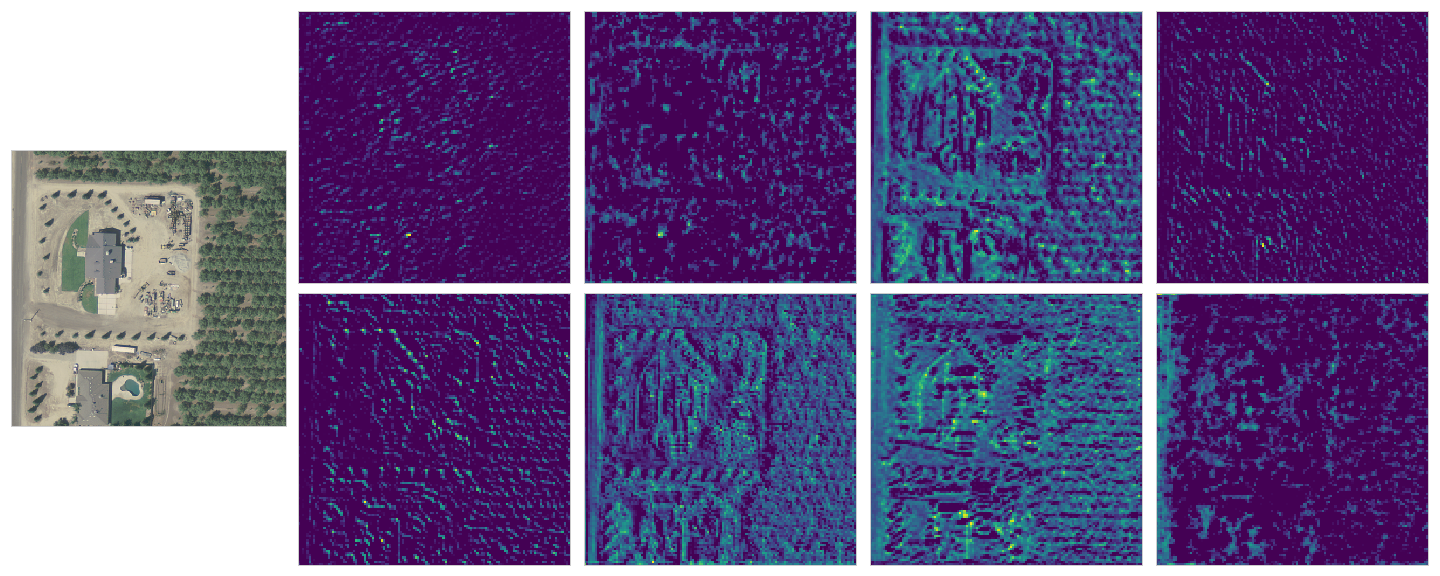
\includegraphics[width=0.9\textwidth]{Figures/activations/agriculture_l2_s1_activation_10.png}
	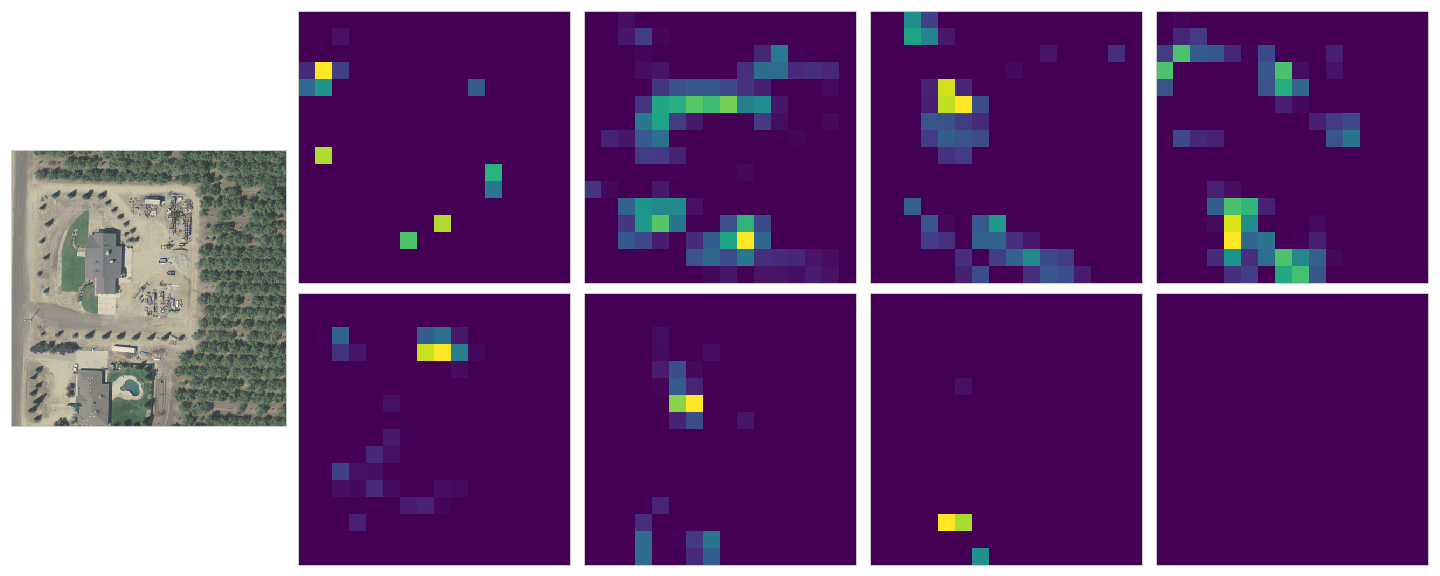
\includegraphics[width=0.9\textwidth]{Figures/activations/agriculture_l2_s1_activation_49.png}
	\captionsetup{width=1\linewidth}
	\caption{\textbf{ResNet activations of an Agriculture image: $10^{th}$ layer (top) and final layer, $49^{th}$ (bottom).}}
	\label{fig:act_agriculture}
\end{figure}

\begin{figure}[H]
	\centering
	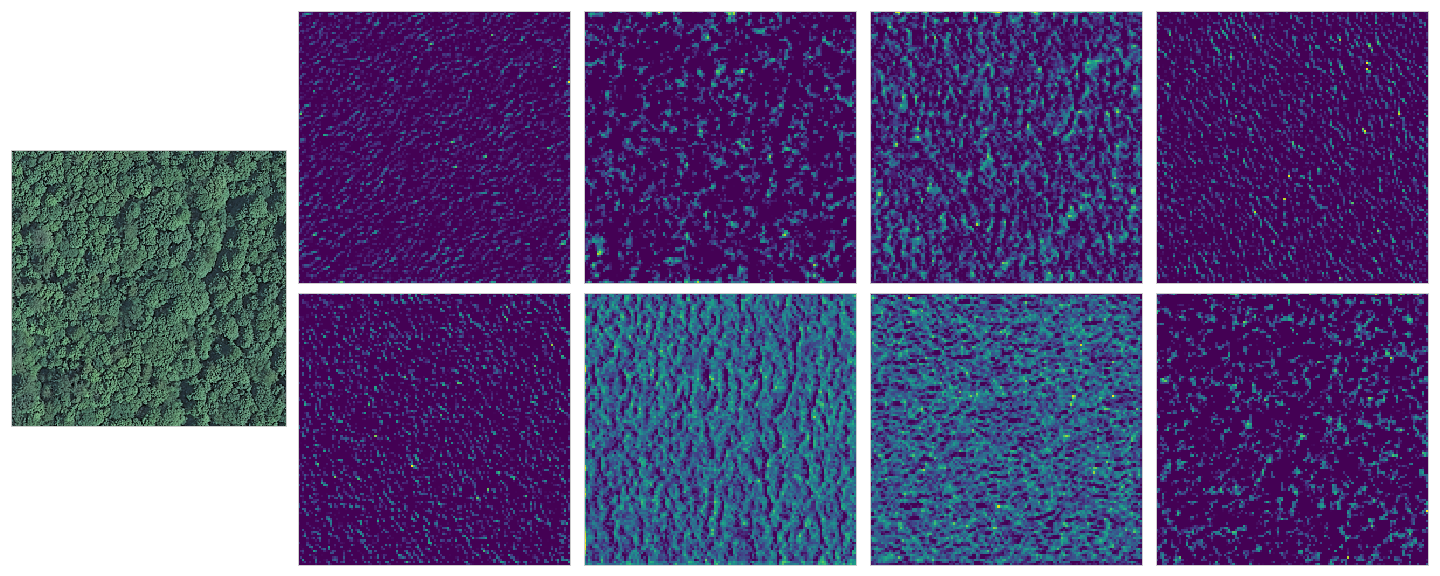
\includegraphics[width=0.9\textwidth]{Figures/activations/forest-woodland_l0_s1_activation_10.png}
	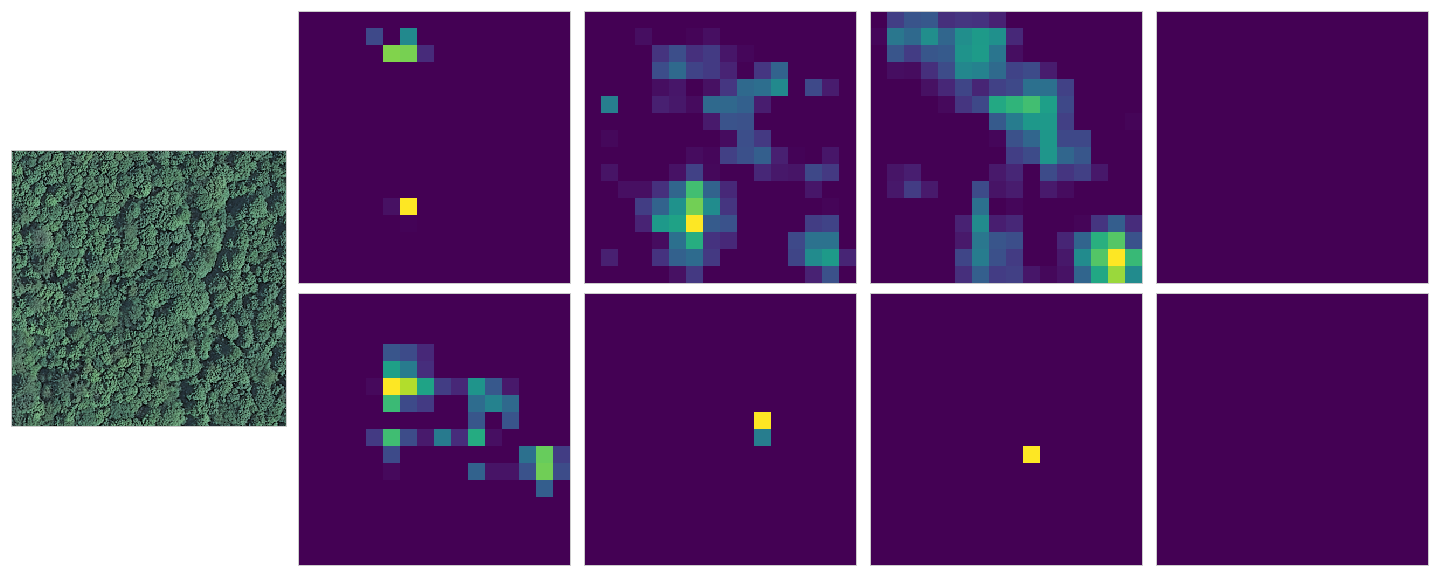
\includegraphics[width=0.9\textwidth]{Figures/activations/forest-woodland_l0_s1_activation_49.png}
	\captionsetup{width=1\linewidth}
	\caption{\textbf{ResNet activations of a Forest-woodland image: $10^{th}$ layer (top) and final layer, $49^{th}$ (bottom).}}
	\label{fig:act_forest_woodland}
\end{figure}

\begin{figure}[H]
	\centering
	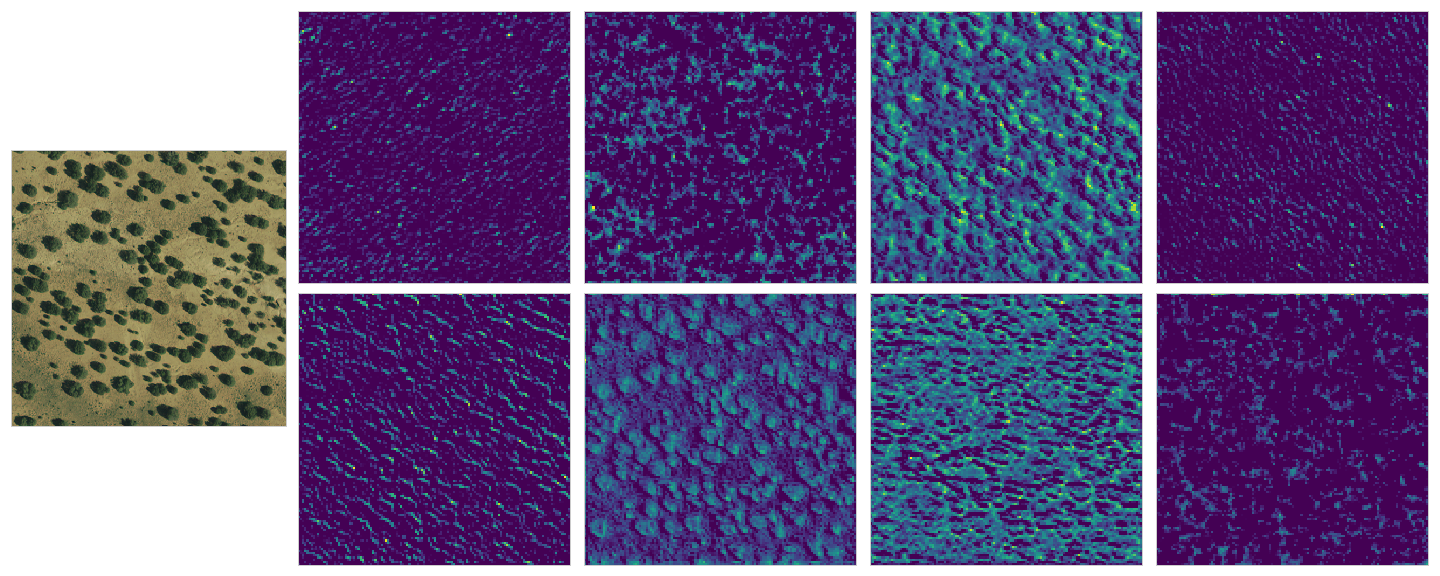
\includegraphics[width=0.9\textwidth]{Figures/activations/semi-desert_l0_s1_activation_10.png}
	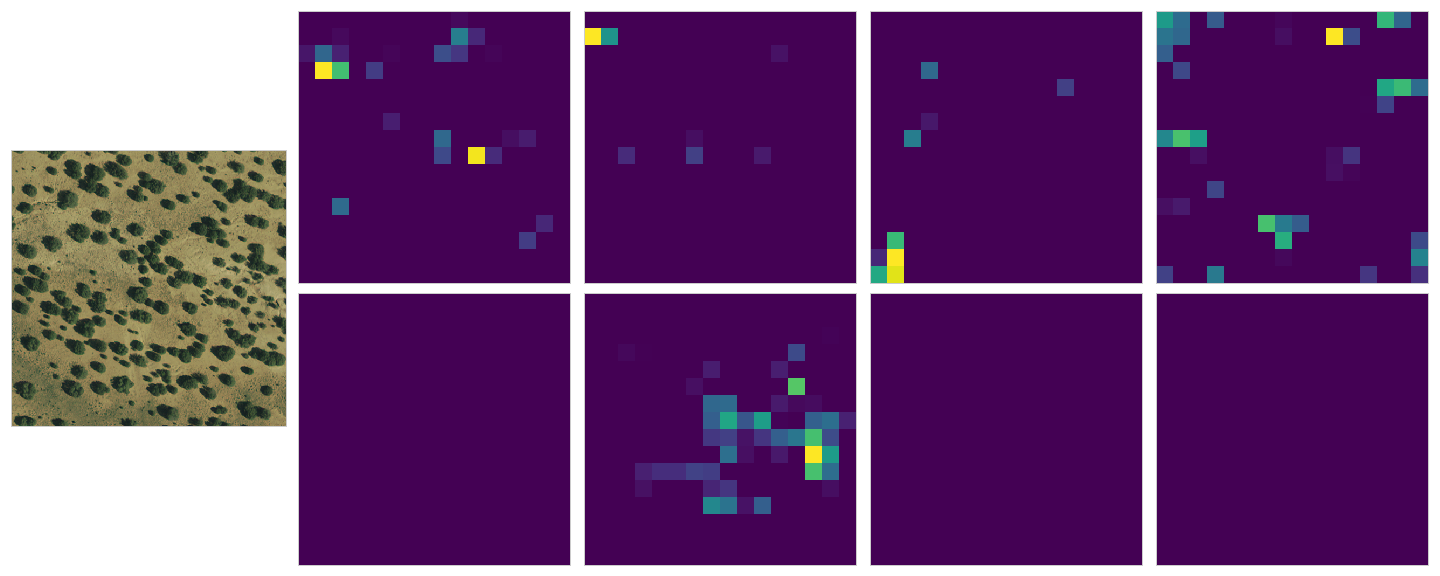
\includegraphics[width=0.9\textwidth]{Figures/activations/semi-desert_l0_s1_activation_49.png}
	\captionsetup{width=1\linewidth}
	\caption{\textbf{ResNet activations of a Semi-desert image: $10^{th}$ layer (top) and final layer, $49^{th}$ (bottom).}}
	\label{fig:act_semi_desert}
\end{figure}

\begin{figure}[H]
	\centering
	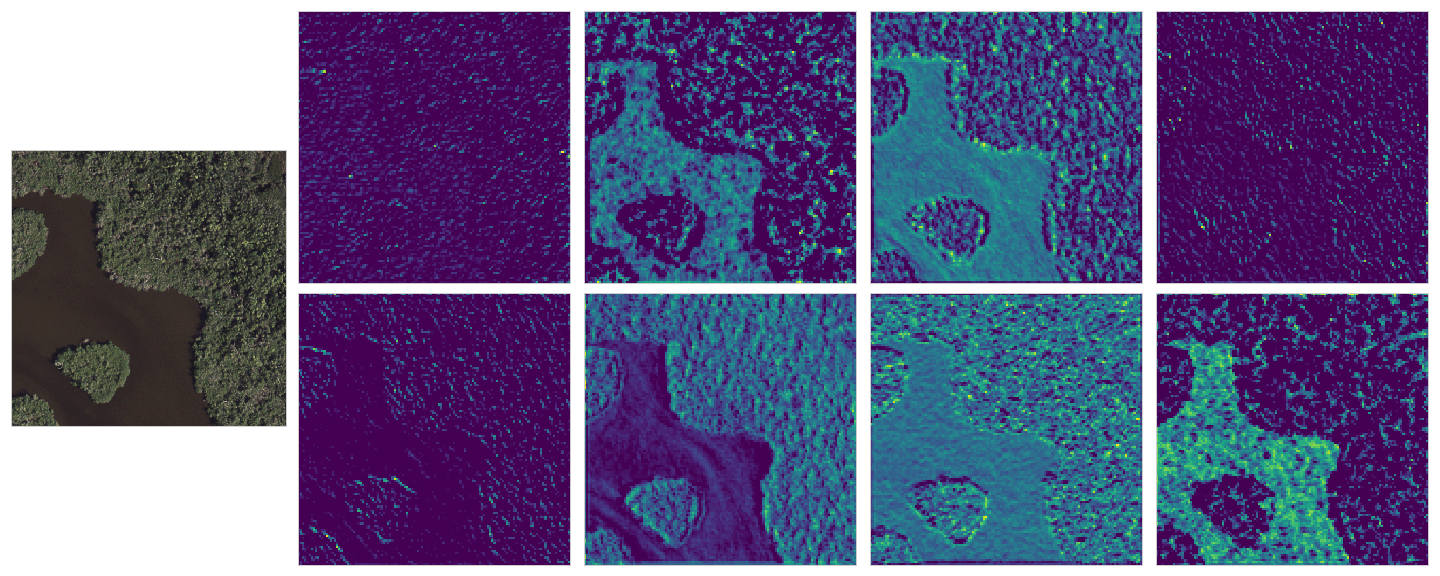
\includegraphics[width=0.9\textwidth]{Figures/activations/shrubland-grassland_l0_s1_activation_10.png}
	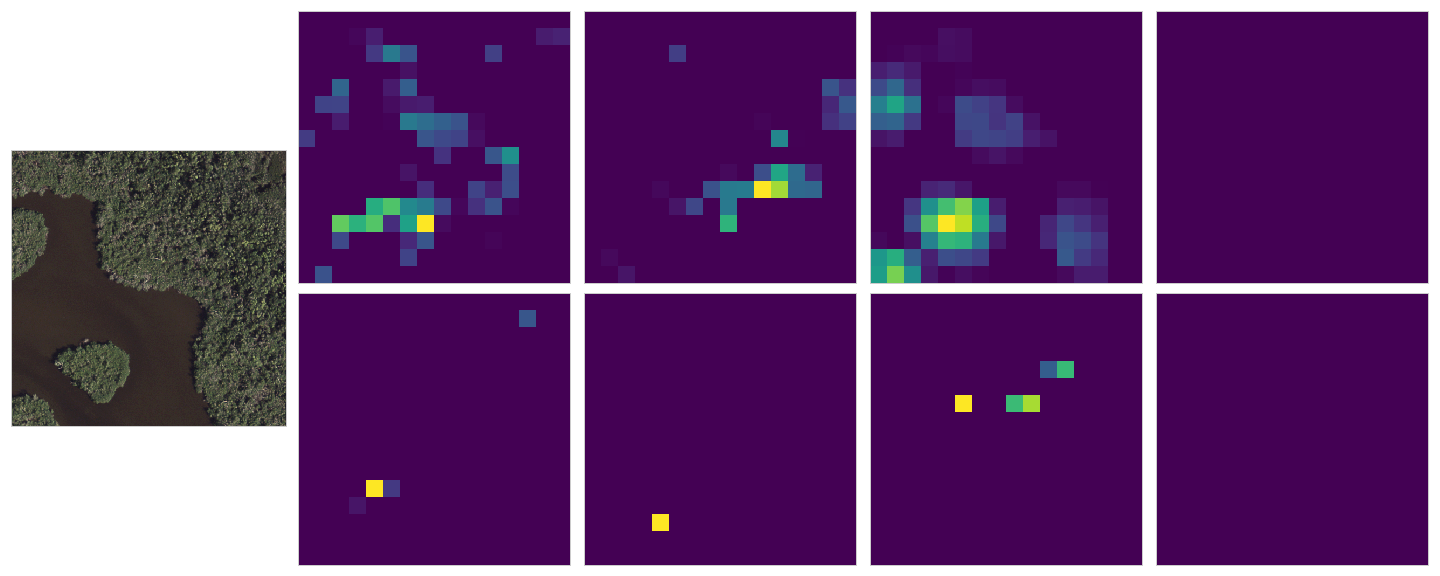
\includegraphics[width=0.9\textwidth]{Figures/activations/shrubland-grassland_l0_s1_activation_49.png}
	\captionsetup{width=1\linewidth}
	\caption{\textbf{ResNet activations of a Shrubland-grassland image: $10^{th}$ layer (top) and final layer, $49^{th}$ (bottom).}}
	\label{fig:act_shrubland_grassland}
\end{figure}


\subsection{Complete architecture}

For our purpose we considered the last ($49^{th}$) activation layer of the ResNet as the features of our images. These features can be extracted and saved on disk in order to speed up the process (as we did), or computed each time, and then passed through a simple fully connected Neural Network.

We terminated the ResNet architecture with a NN that consists of a single dense layer of $100$ or $200$ neurons with ReLU activation, followed by a single dense node with a Sigmoid activation acting as the classifier. This model is trained on the dataset with RMSprop optimizer \parencite{ruder2016} and a binary cross-entropy loss function. The same architecture is used and trained separately for each of the resolutions considered. 

This architecture (see Fig. \ref{fig:transfer_learning}) has been implemented with Python and Keras. Figure \ref{fig:model_keras} shows the model build, while in the following section we describe the complete training pipeline in more detail.

\begin{figure}[h!]
	\centering
	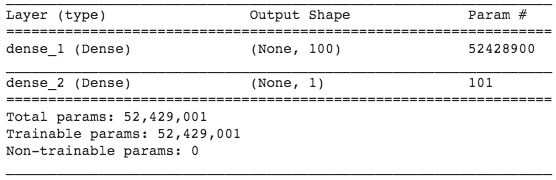
\includegraphics[width=0.8\textwidth]{Figures/model_keras.png}
	\captionsetup{width=1\linewidth}
	\caption{\textbf{Model build with Keras}}
	\label{fig:model_keras}
\end{figure}


\subsection{Training pipeline and experiments}

As introduced in previous chapters, our goal with this model is to study how feasible it is (technically and costly speaking) to detect different kind of human impact on satellite images, and how this detection behaves for different image resolutions. To do so, we build two datasets of annotated images at base resolutions of $0.3m$ and $1m$ (see Chapter \ref{Chapter2}), which we later downgrade to a range of resolutions suitable for our study.

Starting from an image at its base resolution and size ($512\times512$ pixels), the downgrade process consists of downsampling (removing) pixels, so the image becomes smaller. Therefore, this imposes a limit on how far a given dataset can be downgraded, as the CNN ResNet model requires a minimum input size of $32\times32$ pixels due to the application of stride 2 at multiple layers \parencite{ResNetKeras}. Note that during the downsampling process the physical area displayed by the image is not changed. Tables \ref{tab:resolutions_03m} and \ref{tab:resolutions_1m} show the resolutions and sizes considered for the two datasets.

\

\begin{figure}[H]
	\centering
	\begin{tabular}{@{\hskip3pt}r@{\hskip3pt}|@{\hskip3pt}c@{\hskip3pt}@{\hskip3pt}c@{\hskip3pt}@{\hskip3pt}c@{\hskip3pt}@{\hskip3pt}c@{\hskip3pt}@{\hskip3pt}c@{\hskip3pt}@{\hskip3pt}c@{\hskip3pt}@{\hskip3pt}c@{\hskip3pt}@{\hskip3pt}c@{\hskip3pt}@{\hskip3pt}c@{\hskip3pt}@{\hskip3pt}c@{\hskip3pt}@{\hskip3pt}c@{\hskip3pt}@{\hskip3pt}c@{\hskip3pt}@{\hskip3pt}c@{\hskip3pt}@{\hskip3pt}c@{\hskip3pt}@{\hskip3pt}c@{\hskip3pt}@{\hskip3pt}c@{\hskip3pt}}
\textbf{resolution (m)} & 0.3 & 0.6 & 0.9 & 1.2 & 1.5 & 1.8 & 2.1 & 2.4 & 2.7 & 3.0 & 3.3 & 3.6 & 3.9 & 4.2 & 4.5 & 4.8 \\
\midrule
\textbf{size (pixels)} & 512 & 256 & 171 & 128 & 102 & 85 & 73 & 64 & 57 & 51 & 47 & 43 & 39 & 37 & 34 & 32 \\
\end{tabular}

	\captionsetup{width=1\linewidth}
	\caption{\textbf{Relation between resolution and size for the $0.3m$ dataset}. Size is the width (and height) of a square image.}
	\label{tab:resolutions_03m}
\end{figure}

\

\begin{figure}[H]
	\centering
	\begin{tabular}{@{\hskip3pt}r@{\hskip3pt}|@{\hskip3pt}c@{\hskip3pt}@{\hskip3pt}c@{\hskip3pt}@{\hskip3pt}c@{\hskip3pt}@{\hskip3pt}c@{\hskip3pt}@{\hskip3pt}c@{\hskip3pt}@{\hskip3pt}c@{\hskip3pt}@{\hskip3pt}c@{\hskip3pt}@{\hskip3pt}c@{\hskip3pt}@{\hskip3pt}c@{\hskip3pt}@{\hskip3pt}c@{\hskip3pt}@{\hskip3pt}c@{\hskip3pt}@{\hskip3pt}c@{\hskip3pt}@{\hskip3pt}c@{\hskip3pt}@{\hskip3pt}c@{\hskip3pt}@{\hskip3pt}c@{\hskip3pt}@{\hskip3pt}c@{\hskip3pt}}
\textbf{resolution (m)} & 1 & 2 & 3 & 4 & 5 & 6 & 7 & 8 & 9 & 10 & 11 & 12 & 13 & 14 & 15 & 16 \\
\midrule
\textbf{size (pixels)} & 512 & 256 & 171 & 128 & 102 & 85 & 73 & 64 & 57 & 51 & 47 & 43 & 39 & 37 & 34 & 32 \\
\end{tabular}

	\captionsetup{width=1\linewidth}
	\caption{\textbf{Relation between resolution and size for the $1m$ dataset}. Size is the width (and height) of a square image.}
	\label{tab:resolutions_1m}
\end{figure}

\

Next, for each of the datasets and downgraded resolutions we want to train a separate model and assess its performance. To this end, we consider the following pipeline for each of the datasets:

\begin{enumerate}
	\item Load the original images (at the original resolution) from disk along with the human impact labels and categories.
	
	\item Downsample the images to the desired resolution (from the lists in \ref{tab:resolutions_03m} and \ref{tab:resolutions_1m})
	
	\item Compute the ResNet activations (at the $49^{th}$ activation layer) of the resulting downgraded images. These activations can be saved to disk for later use if needed.
	
	\item Consider a stratified KFold split of the dataset (with $8$ splits) for cross-validation. That means, the dataset is split into $8$ sets with labels 0-1 equally distributed. Note that label 1 here represents the class with clear human impact, in contrast to the convention in chapter \ref{Chapter2} (where it was class 2).  Each cross-validation fold consists of around $300$ images for the $0.3m$ dataset, and around $200$ samples for the $1m$ dataset.
	
	\item Train the model (Fig. \ref{fig:model_keras}) separately for each combination of the $7$ training sets considering 30 epochs. The remaining set is used as a validation set to assess the accuracy. After training on all folds, the results of the $8$ experiments are averaged in order to obtain more consistent measures.
	
	\item Repeat the process for all downgraded resolutions.
\end{enumerate}

Note that the splitting parameters of the cross-validation, the model complexity and the training epochs could be further analyzed in order to find the best combination for each of the resolutions tested. Actually, all the experiments consist of training NN models for two datasets, each with $16$ resolutions and $8$ folds per resolution, so every fine-tuning (like changing the size of the NN) implies several executions with some variability on each stage.

Nonetheless, as already mentioned in the introduction, the final goal of the experiments is to have a statistical reference of how well the models can be trained, and not to achieve the highest accuracy for each scenario. In order to do so, a larger dataset would be needed, with more well defined categories and objects, and a clear goal of what needs to be modeled.

The plots in Figures \ref{fig:conv_plots_03m} and \ref{fig:conv_plots_1m} (next pages) display the convergence of some of the models trained, for the different datasets and resolutions (base and lowest resolutions), and showing one of the cross-validation folds only. Also, two architectures for the dense layer have been tested: $100$ neurons and $200$ neurons. 

In general, the NN is able to converge and achieve a good accuracy (as shown in the plots), although for some particular splits of the data, it fails to converge and stays in a low accuracy point (see Figure \ref{fig:bad_convergence_plot}). This is probably due to the fact of having a relative small dataset, makes it difficult to train a complex network. Hence, we apply a threshold of $0.6$ on the accuracy obtained, so these particular folds are not going to be considered when computing the final averaged results.

\

In the next chapter we discuss in much more detail the results obtained from all these experiments.

\

\begin{figure}[h!]
	\centering
	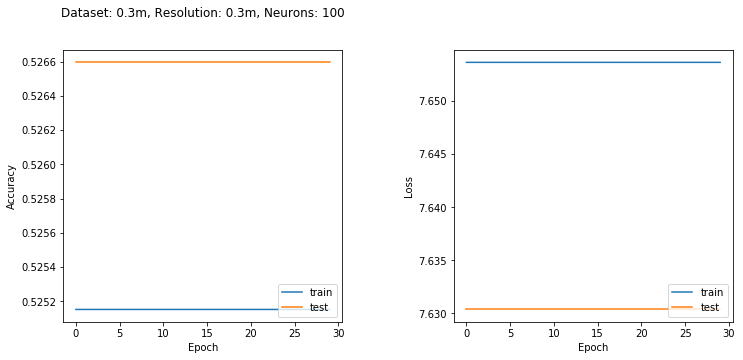
\includegraphics[width=\textwidth]{Figures/results/bad_convergence_plot.png}
	\captionsetup{width=1\linewidth}
	\caption{\textbf{Example of a cross-validation fold for which the model is not able to converge.} The NN weights stay at their initial value during training, without minimizing the loss and resulting in a smaller accuracy.}
	\label{fig:bad_convergence_plot}
\end{figure}

\begin{figure}[h!]
	\centering
	\includegraphics[width=\textwidth]{Figures/results/convergence_plots_03m.png}
	\captionsetup{width=1\linewidth}
	\caption{\textbf{Convergence plots of some experiments on the $0.3m$ dataset, for base ($0.3m$) and lowest ($4.8m$) resolutions, and considering $100$ and $200$ neurons.} The models converge more smoothly for lower resolutions, were there are fewer parameters to be fitted.}
	\label{fig:conv_plots_03m}
\end{figure}

\begin{figure}[h!]
	\centering
	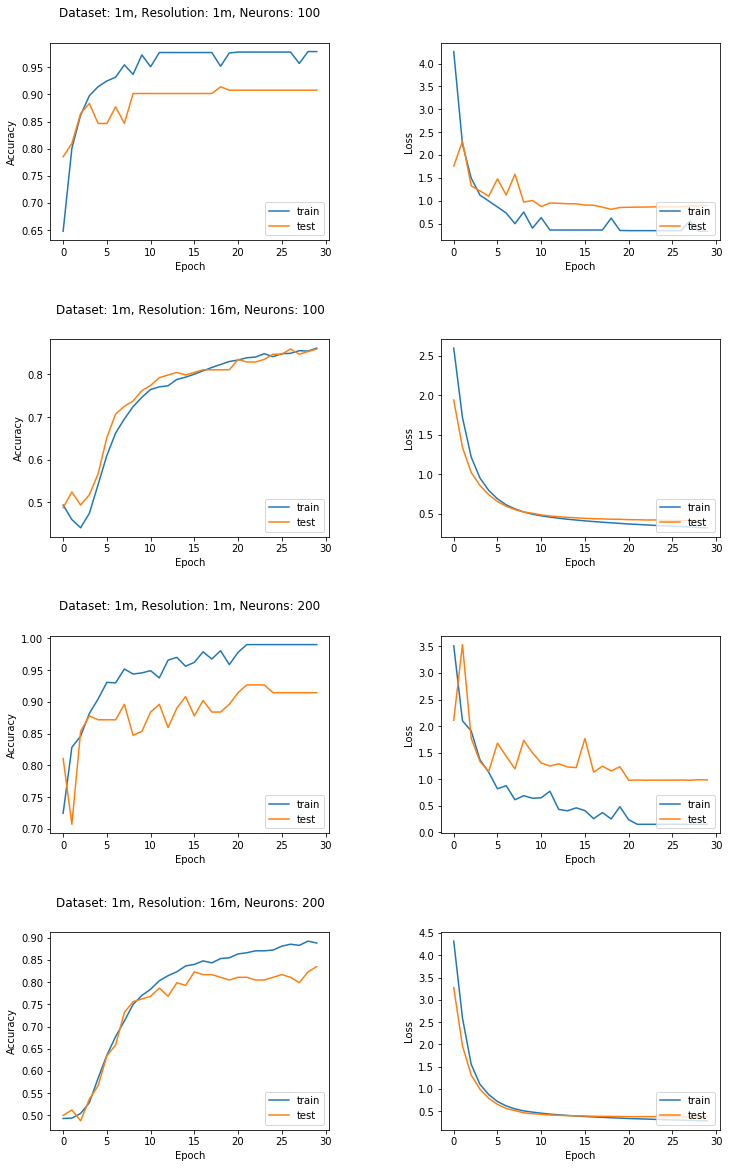
\includegraphics[width=\textwidth]{Figures/results/convergence_plots_1m.png}
	\captionsetup{width=1\linewidth}
	\caption{\textbf{Convergence plots of some experiments on the $1m$ dataset, for base ($1m$) and lowest ($16m$) resolutions, and considering $100$ and $200$ neurons.} The models converge more smoothly for lower resolutions, were there are fewer parameters to be fitted.}
	\label{fig:conv_plots_1m}
\end{figure}
